\documentclass[a4paper,14pt]{extarticle}

\usepackage[T2A]{fontenc}			
\usepackage[utf8]{inputenc}			
\usepackage[english,russian]{babel}

\usepackage[
bookmarks=true, colorlinks=true, unicode=true,
urlcolor=black,linkcolor=black, anchorcolor=black,
citecolor=black, menucolor=black, filecolor=black,
]{hyperref}

\usepackage{color}
\usepackage{caption}
\DeclareCaptionFont{white}{\color{black}}
\DeclareCaptionFormat{listing}{\colorbox{white}{\parbox{\textwidth}{#1#2#3}}}
\captionsetup[lstlisting]{format=listing,labelfont=white,textfont=white}

\usepackage{amsmath,amsfonts,amssymb,amsthm,mathtools} 
\usepackage{wasysym}

%\usepackage[cache=false]{minted}

\usepackage{graphicx}
\usepackage{cmap}
\usepackage{indentfirst}

\usepackage{longtable}

\usepackage{listings} 
\usepackage{fancyvrb}

\usepackage{geometry}
\geometry{left=2cm}
\geometry{right=1.5cm}
\geometry{top=1cm}
\geometry{bottom=2cm}

\setlength{\parindent}{5ex}
\setlength{\parskip}{0.5em}

\usepackage{color}
\usepackage[cache=false, newfloat]{minted}
\newenvironment{code}{\captionsetup{type=listing}}{}
\SetupFloatingEnvironment{listing}{name=Листинг}
 
 
 \begin{document}
 	
 	\def\figurename{Рисунок}
 	
 	\begin{minipage}{0.2\textwidth}
 		
\includegraphics[scale=0.05]{img/bmstu.png}
 	\end{minipage}
 	\begin{minipage}{0.7\textwidth}
 		\small
 		\begin{center}
 			\textbf{Министерство науки и высшего образования Российской Федерации}
 			
 			\textbf{Федеральное государственное бюджетное образовательное учреждение высшего образования «Московский государственный технический университет имени Н.Э. Баумана}
 			
 			\textbf{(национальный исследовательский университет)»}
 			
 			\textbf{(МГТУ им. Н.Э. Баумана)}
 		\end{center}
 	\end{minipage}
 	
 	\vspace*{5mm}
 	
 	\normalsize
 	\begin{flushleft}
 		Факультет: <<Информатика и системы управления>>
 		
 		Кафедра: <<Программное обеспечение ЭВМ и информационные технологии>>
 	\end{flushleft}
 	
 	\vspace*{30mm}
 	
 	\LARGE
 	\begin{center}
 		\textbf{Расчетно-пояснительная записка}
 		
 		%	\textbf{к курсовому проекту на тему:}
 		\textbf{по НИР на тему:}
 		
 		\textbf{<<Метод распознавания звуков в звучащей речи на Естественном Языке>>}
 	\end{center}
 	
 	\vspace*{15mm}
 	
 	\large
 	\begin{flushleft}
 		\textbf{Студент:} Левушкин И. К. \\
 		\textbf{Группа:} ИУ7-72Б \\
 		%        \textbf{Оценка (баллы):} \\
 		\textbf{Научный руководитель:} Градов В.М.
 	\end{flushleft}
 	
 	\vspace*{50mm}
 	
 	\large
 	\begin{center}
 		Москва, 2020 г.
 	\end{center}
 	
 	\thispagestyle{empty}
 	
 	\newpage
 	
 	\tableofcontents
 	\newpage
 	\section*{Введение}
 	\addcontentsline{toc}{section}{Введение}
 	
 	Распознавание речи — одна из самых интересных и сложных задач искусственного интеллекта. Здесь задействованы достижения весьма различных областей: от компьютерной лингвистики до цифровой обработки сигналов.
 	
 	\newpage
 	
 	\section{Аналитический раздел}
 	
 	\subsection{Классический подход к распознаванию речи}
 	
 	Классический подход к распознаванию речи представляет собой последовательность следующих действий (этапов):
 	
 	\begin{itemize}
 		\item Извлечение признаков (Feature Extraction)
 		\item Построение и обучение акустической модели (Acoustic model)
 		\item Декодер, выбирающий наиболее вероятный путь перехода по HCLG-графу:
 		\begin{itemize}
 			\item H модуль на базе HMM
 			\item C модуль контекстной зависимости
 			\item L модуль произношения
 			\item G модуль языковой модели
 		\end{itemize} 
 		\item Rescoring - перевзвешивание гипотез и выдача окончательного результата
 	\end{itemize}
 	
 	\begin{figure}[h!]
 		\begin{center}
 			{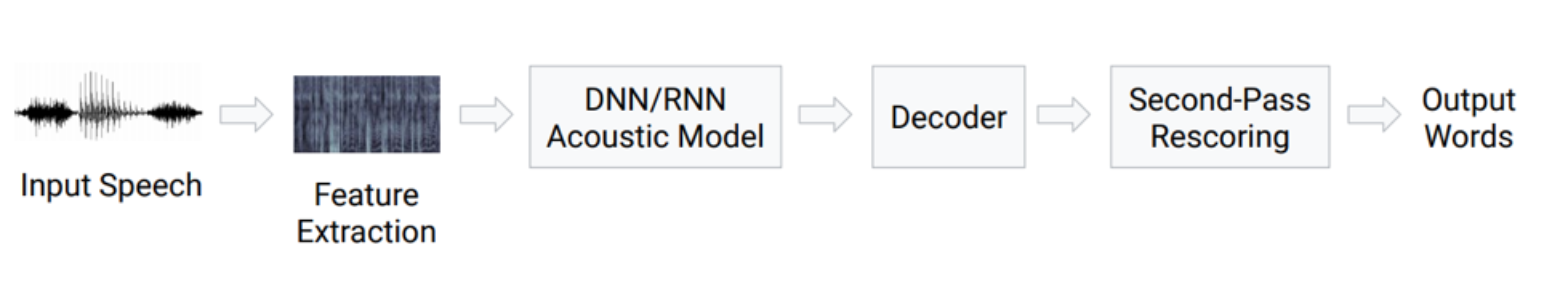
\includegraphics[scale = 0.6]{img/classic.png}}
 			\label{ris:classic}
 		\end{center}
 		\caption{Классический подход.}
 	\end{figure}
 
 	\subsection{Входные данные}
 	
 	Для начала нужно понимать, что наша речь - это последовательность звуков. Звук в свою очередь — это суперпозиция (наложение) звуковых колебаний (волн) различных частот. Волна характеризуются двумя атрибутами — амплитудой и частотой.
 	
 	\begin{figure}[h!]
 		\begin{center}
 			{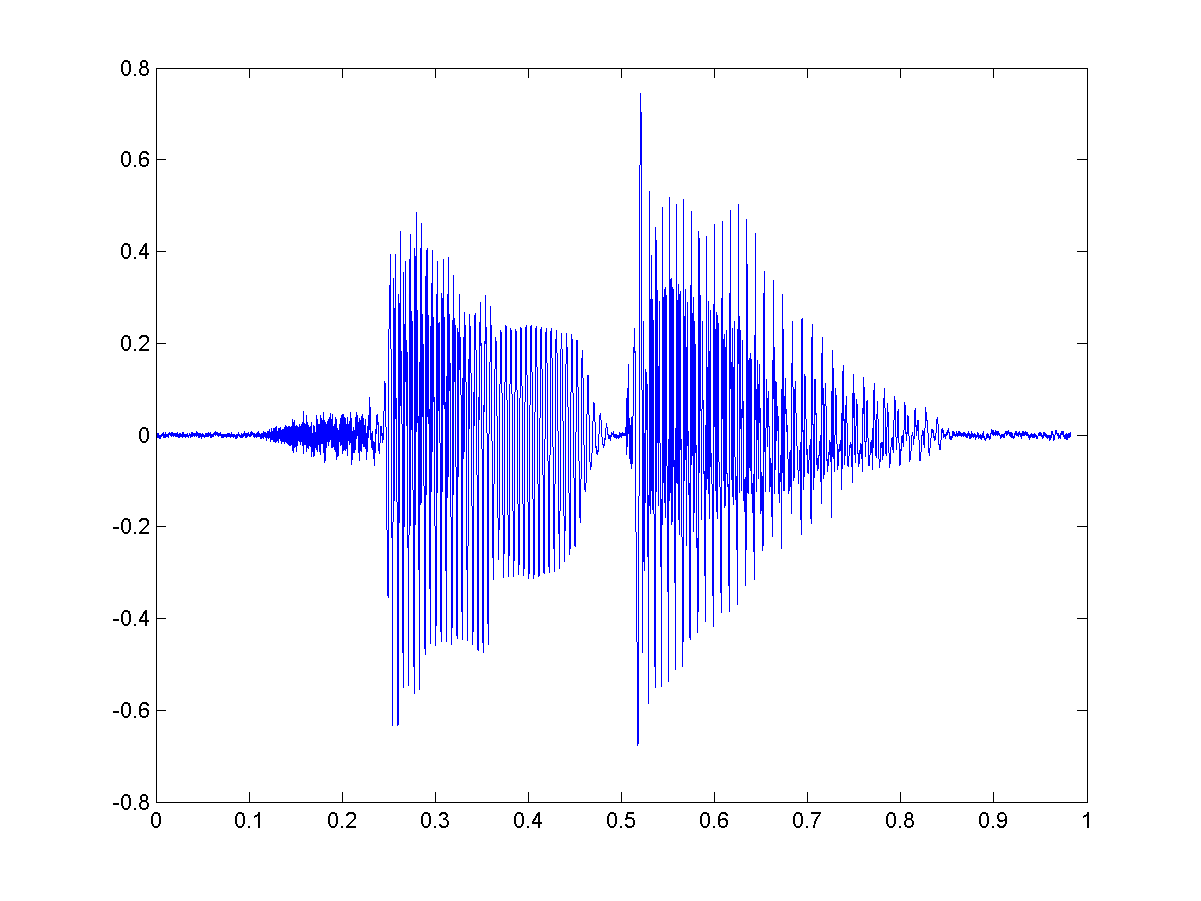
\includegraphics[scale = 0.35]{img/wave.png}}
 			\label{ris:wave}
 		\end{center}
 		\caption{Пример звуковой волны.}
 	\end{figure}
 
 	Другими словами, наши данные - это записанные дорожки аудиофайлов, которые необходимо далее преобразовать в вектор признаков для обучения модели.
 
 	\subsection{Извлечение признаков (Feature Extraction)}
 	
 	Для извлечения признаков из звуковой дорожки необходимо разбить ее на мелкие единицы размером около 10 мс - \textit{фреймы}. Причём фреймы должны идти не строго друг за другом, а <<внахлёст>>. То есть конец одного фрейма должен пересекаться с началом другого.
 	
 	Фреймы являются более подходящей единицей анализа данных, чем конкретные значения сигнала, так как анализировать волны намного удобней на некотором промежутке, чем в конкретных точках. Расположение же фреймов <<внахлёст>> позволяет сгладить результаты анализа фреймов, превращая идею фреймов в некоторое <<окно>>, движущееся вдоль исходной функции (значений сигнала).
 	
 	Разбив дорожку на фреймы, необходимо преобразовать ее в вектор признаков.
 
 	Для такой задачи существует множество способов, но наиболее зарекомендовавший себя среди других - это Мел-частотные кепстральные коэффициенты (Mel-frequency cepstral coefficients).
 	
 	\subsection{MFCC}
 	
 	Mel-frequency cepstral coefficients — это представление энергии спектра сигнала, где mel - единица высоты звука, основанная на восприятии этого звука органами слуха человека.
 	
 	Плюсы его использования:
 	
 	\begin{itemize}
 		\item Используется спектр сигнала (то есть разложение по базису ортогональных [ко]синусоидальных функций), что позволяет учитывать волновую “природу” сигнала при дальнейшем анализе;
 		
 		\item Спектр проецируется на специальную mel-шкалу, позволяя выделить наиболее значимые для восприятия человеком частоты;
 		
 		\item Количество вычисляемых коэффициентов может быть ограничено любым значением, что позволяет <<сжать>> фрейм и, как следствие, количество обрабатываемой информации;
 	\end{itemize}
 
 	Рассмотрим процесс вычисления MFCC коэффициентов для некоторого фрейма.
 	
 	Представим наш фрейм в виде вектора $x[k], 0 <=k<N$, где N - размер фрейма.
 	
 	\subsubsection{Разложение в ряд Фурье}
 	
 	Рассчитываем спектр сигнала с помощью дискретного преобразования Фурье.
 	
 	\[X[k] = \sum_{n=0}^{N - 1} x[n] * e^{-2 \pi i k \frac{n}{N}}, 0 <= k < N\]
 	
 	К полученным значениям применяется оконная функция Хэмминга, чтобы <<сгладить>> значения на границах фреймов.
 	
 	\[H[k] = 0.54 - 0.46 cos(2 \pi k/(N - 1))\]
 	
 	В результате будет вектор следующего вида:
 	
 	\[X[k] = X[k] H[k], 0 <= k < N\]
 	
 	В результате проведенного преобразования по оси Х мы имеем частоту (hz) сигнала, а по оси Y — магнитуду (как способ уйти от комплексных значений):
 	
 	\begin{figure}[h!]
 		\begin{center}
 			{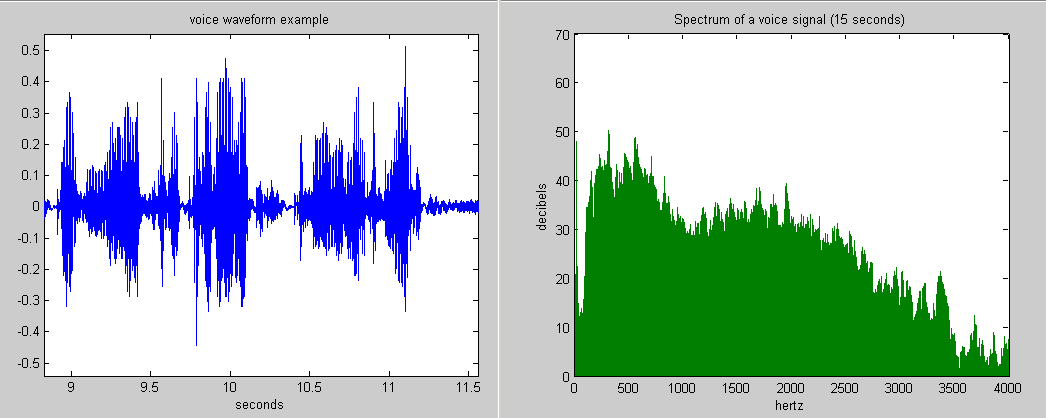
\includegraphics[scale = 0.35]{img/wave_to_freq.png}}
 			\label{ris:wave_to_freq}
 		\end{center}
 		\caption{}
 	\end{figure}
 
 	\subsubsection{Расчет mel-фильтров}
 	
 	Для того, чтобы рассчитать mel-фильтры, необходимо определить, что такое mel.
 	
 	{\bf Mel} — это <<психофизическая единица высоты звука>>, основанная на субъективном восприятии среднестатистическими людьми. Зависит в первую очередь от частоты звука (а так же от громкости и тембра). Другими словами, эта величина, показывающая, на сколько звук определённой частоты <<значим>> для нас.
 	
 	Преобразовать частоту в мел можно по следующей формуле
 	
 	\[M = 1127 log(1 + \frac{F}{700})\]
 	
 	Обратное преобразование выглядит следующим образом
 	
 	\[F = 700 (e^{\frac{M}{1127} - 1})\]
 	
 	Ниже приведен график зависимости mel от частоты
 	
 	\begin{figure}[h!]
 		\begin{center}
 			{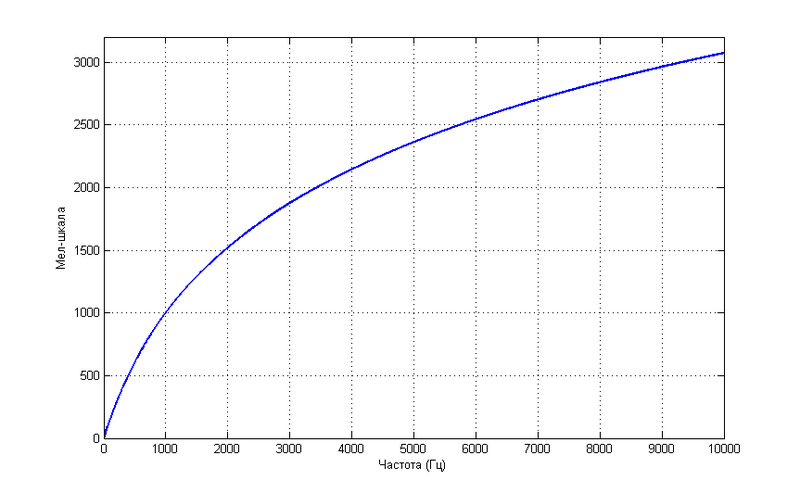
\includegraphics[scale = 0.35]{img/freq.png}}
 			\label{ris:freq}
 		\end{center}
 		\caption{}
 	\end{figure}
 
 	\subsection{Применение фильтров, логарифмирование энергии спектра}
 	
 	Применение фильтра заключается в попарном перемножении его значений со значениями спектра. Результатом этой операции является mel-коэффициент.
 	
 	\[S[m] = log(\sum_{k=0}^{N - 1} |X[k]|^2 H_m[k]), 0 <= m < M\]
 	
 	Необходимо применить mel-фильтры не к значениям спектра, а к его энергии. После чего прологарифмировать полученные результаты. Считается, что таким образом понижается чувствительность коэффициентов к шумам.
 	
 	\subsection{Косинусное преобразование}
 	
 	Дискретное косинусное преобразование (DCT) используется для того, чтобы получить  кепстральные коэффициенты.
 	
 	Делается это, чтобы пронормировать полученные результаты, повысив значимость первых коэффициентов и уменьшив значимость последних.
 	
 	Ниже используется DCTII без домножений на scale factor ($\sqrt{\frac{2}{N}}$).
 	
 	\[C[l] = \sum_{m=0}^{M - 1}S[m] cos(\pi l (m + \frac{1}{2})/M), 0 <= l < M\]
 	
 	На выходе имеем для каждого фрейма набор из M mfcc-коэффициентов, которые могут быть использованы для дальнейшего анализа.
 	
 	\subsection{Акустическая модель}
 	
 	В акустической модели самыми распространенными подходами являются:
 	\begin{itemize}
 		\item скрытые марковские модели (CMM);
 		\item глубокие нейронные сети (DNN).
 	\end{itemize}
 	
 	\newpage
 	
 	\section{Конструкторский раздел}
 	
 	\subsection*{Выводы по конструкторскому разделу}
 	
 	\newpage
 	
 	\section{Технологический раздел}
 	
 	\subsection*{Выводы по технологическому разделу}
 	
 	\newpage
 	\section*{Заключение}
 	\addcontentsline{toc}{section}{Заключение}
 	
 	\newpage
 	
 	\addcontentsline{toc}{section}{Список используемой литературы}
 	\begin{thebibliography}{5}
 		\bibitem{yandex}
 		Распознавание речи от Яндекса. Под капотом у Yandex.SpeechKit [Электронный ресурс]. – Режим доступа: 
 		https://m.habr.com/ru/company/yandex/blog/198556/, 
 		свободный – (20.12.2020)
 		\bibitem{speech}
 		Понижаем барьеры на вход в распознавание речи [Электронный ресурс]. – Режим доступа: 
 		https://m.habr.com/ru/post/494006/, 
 		свободный – (20.12.2020)
 		\bibitem{speech_3}
 		A Fast, Extensible Toolkit for Sequence Modeling [Электронный ресурс]. – Режим доступа: 
 		https://arxiv.org/pdf/1904.01038.pdf, 
 		свободный – (20.12.2020)
 		\bibitem{speech_2}
 		Мел-кепстральные коэффициенты (MFCC) и распознавание речи [Электронный ресурс]. – Режим доступа: 
 		https://habr.com/ru/post/140828/, 
 		свободный – (20.12.2020)
 		\bibitem{speech_for_noob}
 		Распознавание речи для чайников
 		 [Электронный ресурс]. – Режим доступа: 
 		https://habr.com/ru/post/226143/, 
 		свободный – (20.12.2020)
 		
 	\end{thebibliography}
 
\end{document}